% Chapter Template
%\usepackage{subfig}
\chapter{Estado del Arte} % Main chapter title

\label{Chapter2} % Change X to a consecutive number; for referencing this chapter elsewhere, use \ref{ChapterX}

%----------------------------------------------------------------------------------------
%	SECTION 1
%----------------------------------------------------------------------------------------

\section{An\'alisis de im\'agenes de la retina}

El an\'alisis de im\'agenes de la retina es de gran importancia para la detecci\'on de enfermedades del ojo.
El avance tecnol\'ogico permiti\'o obtener im\'agenes de la retina de mayor calidad, lo que beneficia que el analisis de estas permita la detecci\'on precoz de enfermedades con mayor precisi\'on, favoreciendo la disminuci\'on del porcentaje de personas con ceguera debido a enfermedades sistemicas o retinales. 

Existen muchas ventajas en el uso del an\'alisis de imagen digital para cuantificar la extensi\'on de la patolog\'ia de la retina en enfermedades vasculares, retinopat\'ia diab\'etica, degeneraci\'on macular asociada a la edad, y otras condiciones. Los beneficios clave incluyen la accesibilidad inmediata, visualizaci\'on, sistemas de gesti\'on de im\'agenes que permiten el seguimiento de la progresi\'on de la enfermedad mediante la revisi\'on de im\'agenes secuenciales, y la educaci\'on del paciente. Al mismo tiempo las im\'agenes capturadas, tienen una  gran resoluci\'on y se pueden visualizar en una pantalla tan pronto como se obtienen, y  permitiendo detectar y corregir cualquier error en el proceso fotogr\'afico a la vez. \cite{cunha2004blood}


%-----------------------------------
%	SUBSECTION 1
%-----------------------------------
\subsection{Introducci\'on}

La retina es un tejido en capas que recubre el interior del ojo, permitiendo la conversión de la luz entrante en señales neuronales adecuadas para su posterior procesamiento por parte de la corteza visual del cerebro. La misma está sostenida por el epitelio pigmentario retinal, la coroide y la esclera.
La estructura anatómica del ojo se compone básicamente por la córnea (transparente), la esclera (normalmente blanca), el iris (que da color al ojo) y la pupila. Todas estas partes son visibles desde el exterior, y son las responsables de permitir la visión: un rayo de luz pasa a través de la córnea, que enfoca parcialmente la imagen, luego pasa por la cámara anterior, la pupila (que hace las veces de lente y enfoca aún más la imagen), la vítrea y por último es enfocado en la retina.

\begin{figure}[H]
	{
	\centering
	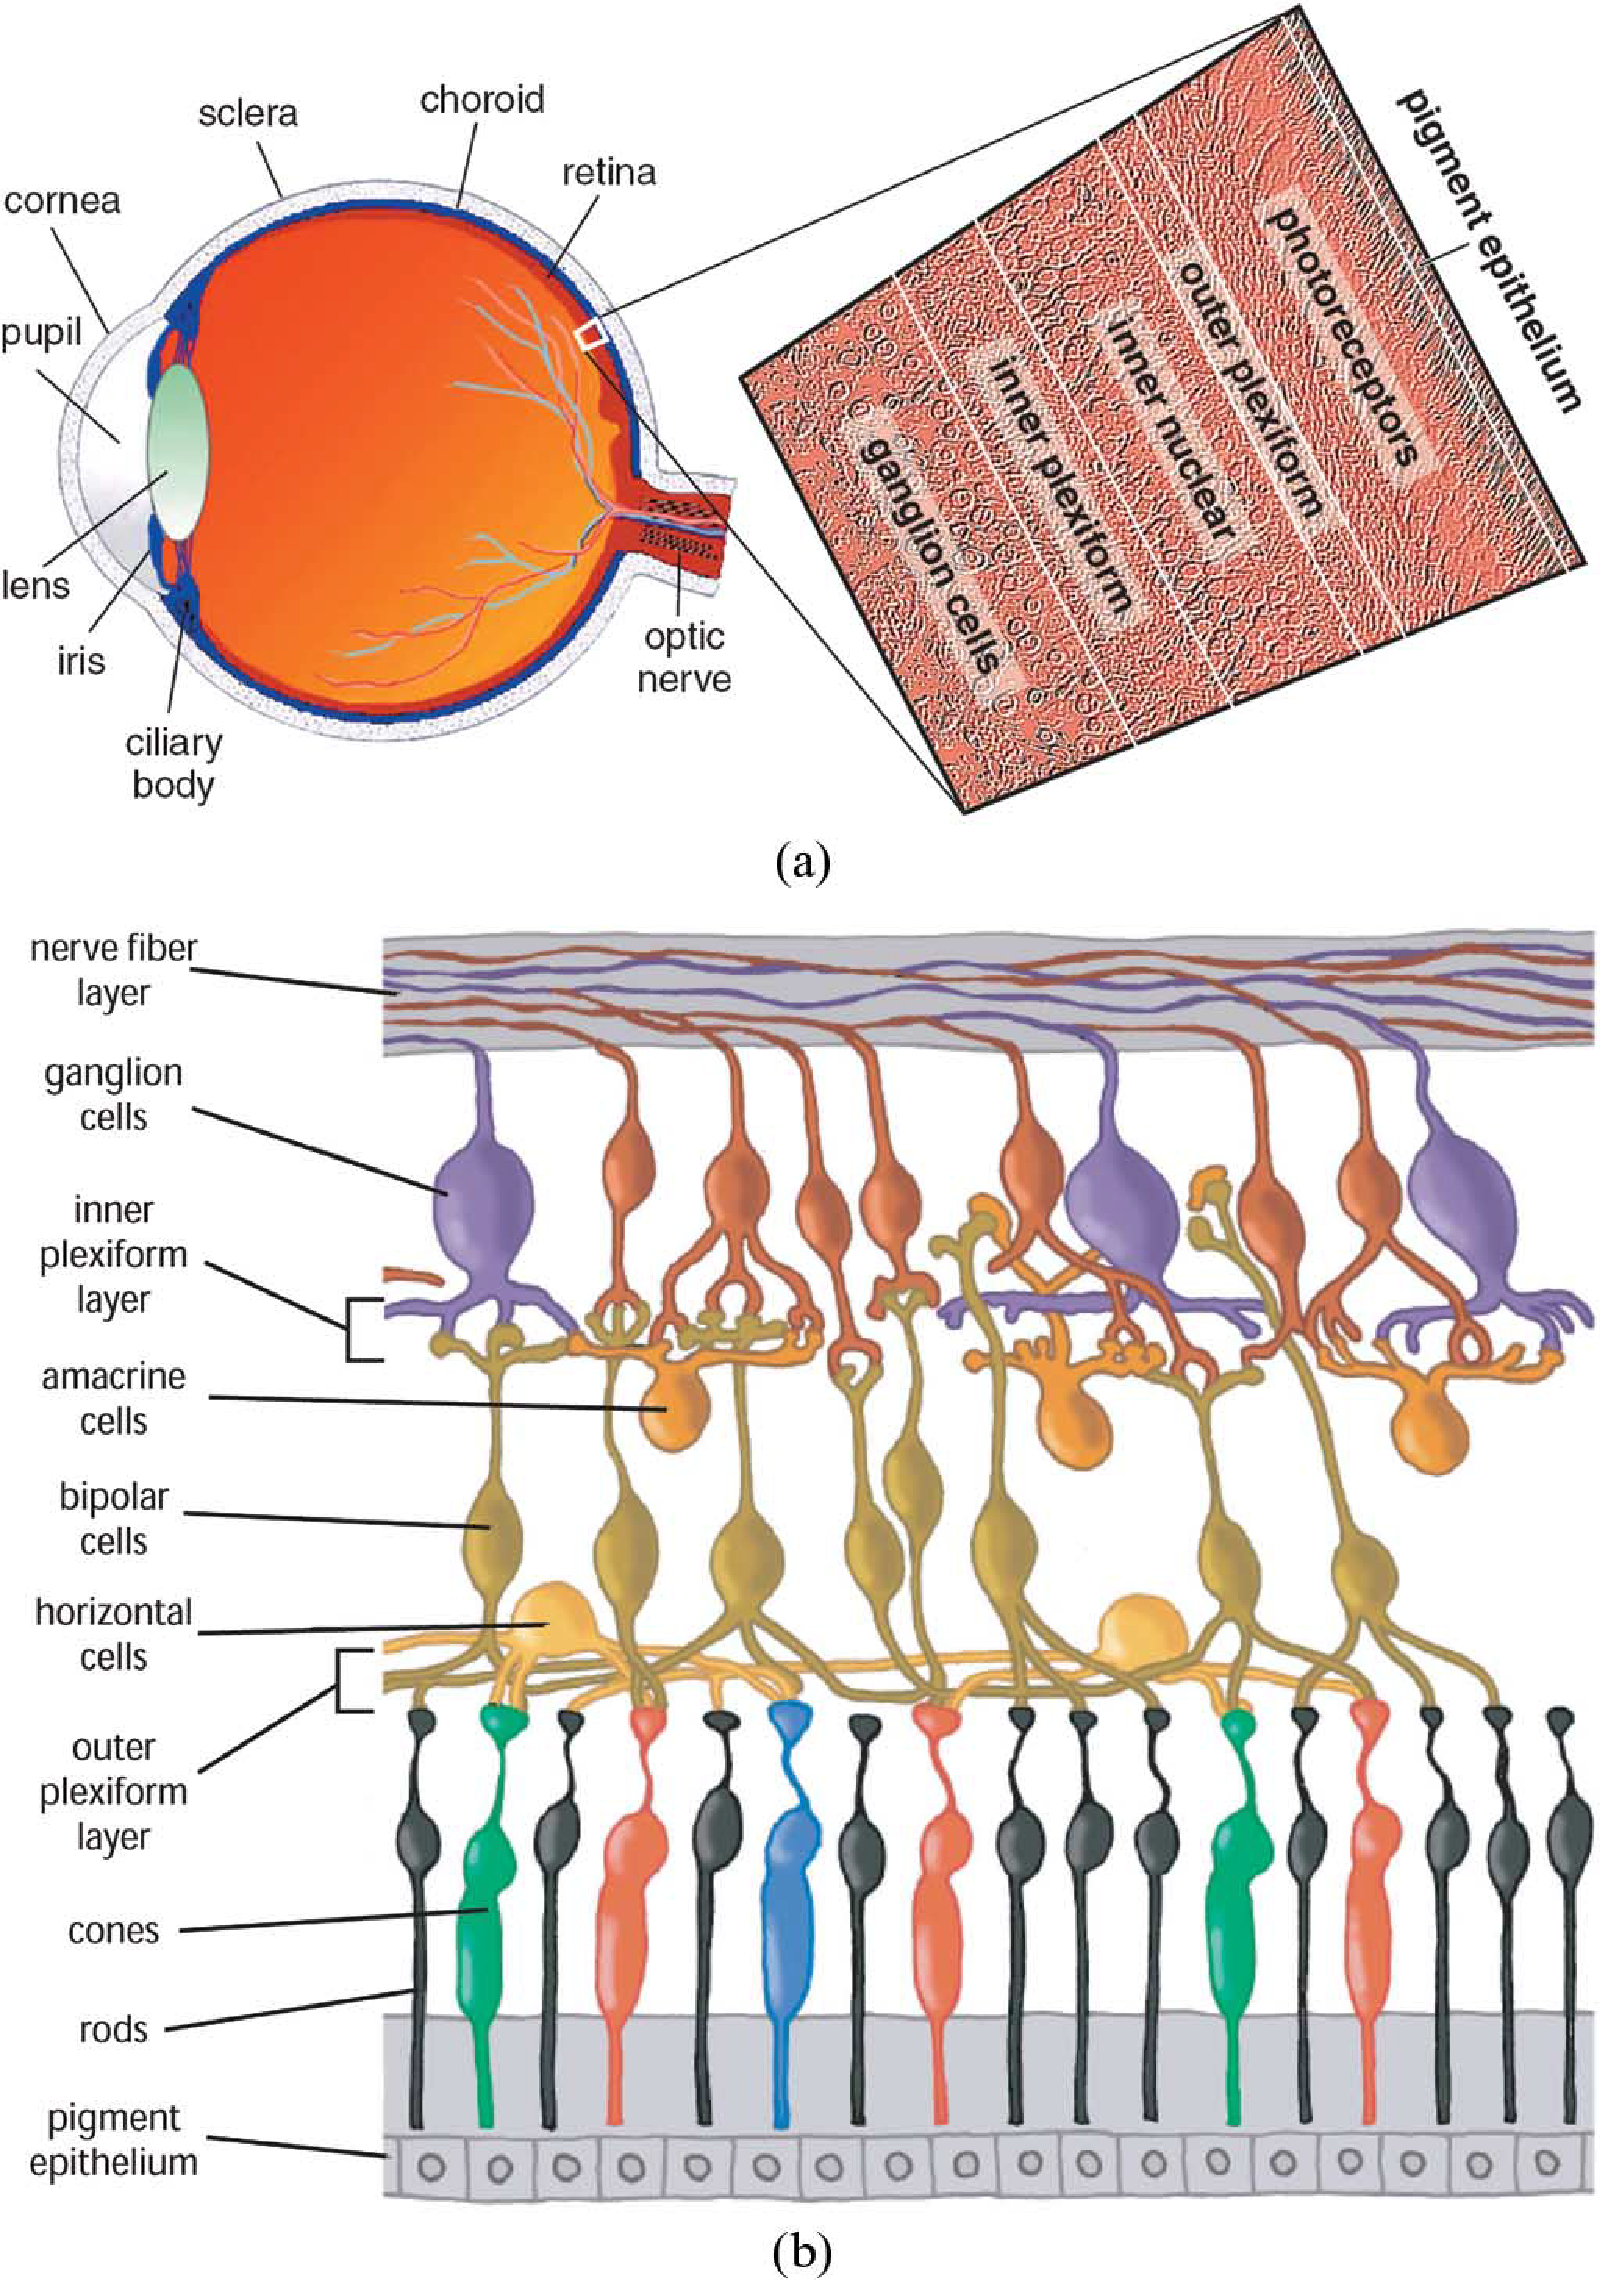
\includegraphics[width=0.75\textwidth]{Figures/ojo}
	\caption[Anatom\'ia del ojo 0-200]{\'Anatom\'ia del ojo. Ilustraci\'in de la anatom\'ia del ojo y capas de la retina [2], [3]. (A) Vista transversal del ojo y sus estructuras principales. La retina es un tejido delgado transparente que recubre la parte posterior del ojo y se compone de un n\'umero de capas, como se ilustra en la parte ampliada. (B) Representaci\'on esquem\'atica de las capas celulares de la retina. (a) Ilustraci\'on bidimensional de la anatom\'ia del ojo. (b)Representaci\'on esquem\'atica de las capas de la retina. Ejemplos de Kolb [3] utilizado con el permiso de Sigma Xi, The Scientific Sociedad de Investigación, Research Triangle Park, Carolina del Norte.}
	\label{fig:AnatomiaDelOjo}
	}
\end{figure}	

Durante la \'ultima d\'ecada, la fotograf\'ia digital a color ha sido reconocida como una modalidad aceptable para documentar el aspecto de la retina, ya que proporciona informaci\'on vital sobre la salud del paciente de la parte sensorial del sistema visual. La segmentaci\'on y el an\'alisis de im\'agenes de la retina se pueden utilizar para detectar el riesgo patol\'ogico o da\~nos, y asistir en el diagn\'ostico. 

El avance en la tecnologia aplicada en las imagenes digitales y  el aumento de la potencia de c\'alculo en dispositivos de procesamiento digital, presentan la posibilidad de utilizar estas tecnolog\'ias en oftalmolog\'ia. La microvasculatura retinal es \'unica, ya que es la \'unica parte de la circulaci\'on humana que puede ser visualizada directamente de forma no invasiva in vivo, fotografiando f\'acilmente el ojo, permitiendo el an\'alisis de las im\'agenes digitales. \cite{patton2006retinal}


T\'ecnicas de procesamiento de imágenes, análisis y visión a traves de dispositivos computacionales se encuentran hoy en d\'ia en todos los campos de la ciencia m\'edica. Estas técnicas son especialmente relevantes para la oftalmología moderna, un campo que depende en gran medida de los datos visuales. Las im\'agenes de la retina son ampliamente utilizadas por ofatalm\'ologos para fines de diagn\'ostico. Sin embargo, estas im\'agenes a menudo necesitan mejoras visuales antes de determinar un an\'alisis digital de riesgo patol\'ogico o la detecci\'on de da\~nos. 
(Lo anterior referencia a -> Marrugo2011)

En el modo tradicional de diagn\'ostico, los oftalm\'ologos examinan las im\'agenes de la retina, buscan las posibles anomal\'ias y entregan un diagn\'ostico. El procesamiento y ana\'lisis de la retina autom\'atico permite ahorrar carga de trabajo y puede ayudar a lograr una detecci\'on mas objetiva a los oftalm\'ologos. Se han hecho esfuerzos para extraer estructuras normales y anormales en im\'agenes de la retina de forma autom\'atica y robusta. La aplicaci\'on de t\'ecnicas de procesamiento de im\'agenes por computadora, para el an\'alisis de las im\'agenes de la retina comenz\'o aproximadamente hacia 1974 [1]. Desde entonces, mucho investigadores han presentado inter\'es en el tema, y han tenido que afrontar diversas dificultades, principalmente los ruidos, iluminaci\'on desigual y la variaci\'on entre los individuos. \cite{li2004automated}


Las enfermedades que pueden manifestarse en el ojo pueden ser b\'asicamente de dos tipos, del ojo en s\'i mismo o sist\'emicas. Existen un conjunto de las mismas que pueden ser detectadas a trav\'es de la captura y el an\'alisis de im\'agenes de distintas estructuras de la retina. Las mismas pueden ser originadas, ya sea, en el ojo mismo, en el cerebro o en el sistema cardiovascular.
Dentro de las enfermedades que pueden diagnosticarse a trav\'es del an\'alisis de im\'agenes de la retina, se encuentra la retinopat\'ia diab\'etica (DR), una complicaci\'on de la Diabetes Mellitus, que afecta a un tercio de los diab\'eticos  y es la principal causa de p\'erdida de visi\'on en personas de edad avanzada,  y sigue siendo una de las principales causas de ceguera evitable. El edema macular diab\'etico (DME), caracterizado por el aumento de la permeabilidad vascular y la deposici\'on de exudados duros en la retina central, puede desarrollarse en cualquier etapa de la DR y aflige a 21 millones de personas en el mundo.  A trav\'es de ex\'amenes peri\'odicos de la vista, la p\'erdida de la visi\'on relacionada con la diabetes se puede prevenir en el 98\% de los casos.
(Lo anterior referencia a -> g0h2016) 
Otra de las enfermedades diagnosticable mediante el an\'alisis de im\'agenes ret\'inales es la degeneraci\'on macular asociada a la edad (DMAE), la cual es la causa mas frecuente de ceguera en pa\'ises desarrollados en personas mayores de 50 anos. Una de las principales medidas para definir la gravedad de la DMAE, es el an\'alisis de derrames, alteraciones pigmentarias, atrofia geogr\'afica  y neovascularizaci\'on coroidea a partir de la proyecci\'on de im\'agenes de fondo de ojo, la tomograf\'ia de coherencia \'optica (OCT) y otras modalidades. Cada una de estas modalidades de imagen tienen puntos fuertes y puntos d\'ebiles para detectar, capturar y / o cuantificar diferentes patolog\'ias. Los tratamientos actuales para la DMAE no pueden curar o revertir la p\'erdida de la visi\'on. Sin embargo, el estudio de las enfermedades oculares relacionadas con la edad, mostr\'o que la suplementaci\'on con vitamina antioxidante espec\'ifica reduce el riesgo de progresi\'on de etapas intermedias, siendo una estrategia preventiva en pacientes correctamente identificados. De este modo la identificaci\'on temprana de pacientes con DMAE es importante para diseñar e implementar estrategias preventivas para el tratamiento del DMAE, y determinar su relaci\'on coste-eficacia. Mediante la teleoftalmolog\'ia o la telemedicina en combinaci\'on con la asistencia de una computadora o dispositivo, se puede realizar el an\'alisis de comunidades alejadas de zonas urbanas o situadas en zonas de riesgo, permitiendo identificar a individuos que padezcan alguna patolog\'ia retinal, en una etapa temprana, a modo de prevenci\'on. \cite{kanagasingam2014progress}


Actualmente existen diversas \'areas de investigación activas en lo que respecta a la imagenología de la retina. Algunas de las \'areas se centran en la b\'usqueda de herramientas rentables, f\'aciles de usar y portables, que asistan en el análisis y procesamiento de las imágenes. Por otro lado CONSULTAR IMAGENES FUNCIONALES. Adaptive Optics o \'optica adaptativa, es otra \'area que se encarga de la utilizaci\'on de lentes para corregir las fallas de frente de onda de la luz reflejada desde la retina, permitiendo la obtenci\'on de celulas individuales o estructuras celulares.
Longer Wavelength OCT Imaging o longitud de onda m\'as larga, realiza investigaciones para el desarrollo de los l\'aseres de baja coherencia de c\'odigo de barrido con longitudes de ondas centrales mayores. Algunos de estos prototipos ya son capaces de resolver los detalles en la coroides y la l\'amina cribosa.

%-----------------------------------
%	SUBSECTION 2
%-----------------------------------

\subsection{Fotograf\'ias de fondo de ojo}

Existen diversas formas de poder observar y analizar la anatom\'ia del ojo, a trav\'es de im\'agenes m\'edicas. 
Una de las modalidades de imagen m\'edica que permite explorar el interior del ojo es la de la imagen de fondo de ojo. La misma consiste en  una representaci\'on 2D del tejido retinal semitransparente 3D, proyectado en el plano de obtenci\'on de la imagen, que se obtiene usando la luz reflejada en el tejido.
Para realizar la captura del fondo de ojo, se dilata la pupila con f\'armacos que se depositan en forma de gotas en la superficie ocular; as\'i, el oftalm\'ologo puede ver con facilidad el interior del globo ocular con un aparato que se llama oftalmoscopio. El oftalmoscopio consiste en un aparato formado por una serie de espejos y cristales que alumbran la retina del ojo sin que la luz se refleje. Si no fuese por el oftalmoscopio la luz provocar\'ia destellos y no se podría ver el fondo de ojo de manera correcta, algo parecido a lo que sucede cuando el flash de una cámara de fotos saca los ojos en color rojo. Esta modalidad no es invasiva, y su costo es menor a la angiografía y la OCT dado que la c\'amara que se necesita para capturar la imagen del ojo es una c\'amara digital convencional.
Adem\'as de facilitar la detecci\'on de enfermedades oculares, las im\'agenes de fondo de ojo permiten detectar tres tipos de lesiones oculares. 

La exploraci\'on del fondo de ojo se realiza para visualizar a trav\'es de la pupila la porci\'on posterior e interior del ojo. Gracias a este procedimiento pueden observarse diferentes estructuras internas del globo ocular: m\'acula, retina y papila \'optica entre otras. Tambi\'en es posible visualizar directamente los vasos sangu\'ineos de la retina.
Para realizar la captura, se utiliza una c\'amara digital encargada de tomar la im\'agen del interior del ojo. Se utiliza un oftalmoscopio de baja potencia que se conecta con la c\'amara digital, este diseño realiza la captura de la fotograf\'ia del fondo del ojo y utiliza la luz del espectro visible para obtener im\'agenes de la estructura de la retina in vivo. En im\'agenes en color, las intensidades de imagen representan la cantidad de longitudes de ondas rojas, verdes y azules reflejadas, como se determina por la sensibilidad espectral del sensor. Dado que el nivel de luz ambiental crea insuficiente iluminaci\'on reflejada por la imagen digital, la iluminaci\'on interior debe ser proyectada en el ojo, y la luz reflejada por la retina debe volver al plano pupilar. Es decir, que se debe proyectar un haz de luz (flash) sobre el ojo, para iluminar el \'organo ocular y obtener una mejor imagen del fondo del ojo. \cite{kanagasingam2014progress}



\begin{figure}[H]
    \centering
    \begin{subfigure}[b]{0.3\textwidth}
				\centering
        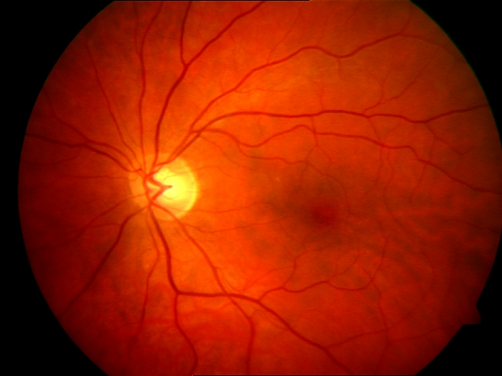
\includegraphics[height=3cm\textwidth]{./Figures/imagesARIA.png}
        \caption{Aria}
        \label{fig:Aria}
    \end{subfigure}
    \begin{subfigure}[b]{0.3\textwidth}
				\centering
        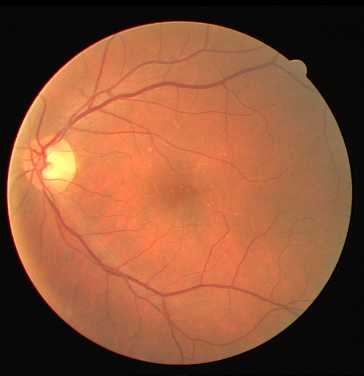
\includegraphics[height=3cm\textwidth]{./Figures/imagesDRIVE.png}
        \caption{Drive}
        \label{fig:Drive}
    \end{subfigure}
    \begin{subfigure}[b]{0.3\textwidth}
				\centering
        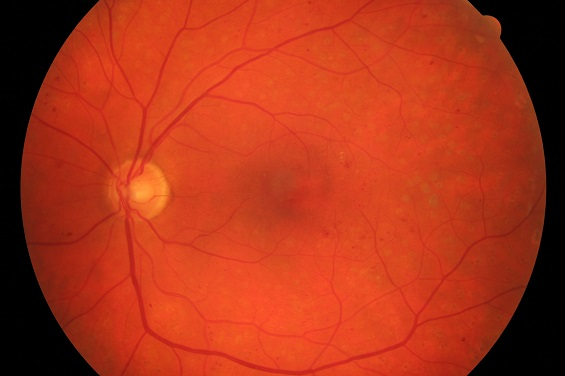
\includegraphics[height=3cm\textwidth]{./Figures/imagesHRF.png}
        \caption{Hrf}
        \label{fig:Hrf}
    \end{subfigure}        
    \label{fig:Imagenes de fondo de ojo}
    \caption{(A) (B) (C)}
\end{figure}

El Instituto Nacional del Reino Unido (NICE) establece que una prueba de cribado de RD debe tener la sensibilidad y la especificidad de al menos el 80\% y 95\%, respectivamente, con una tasa de fallo t\'ecnico inferior al 5\%. El m\'etodo de la fotograf\'ia est\'andar para la detecci\'on de DR es la fotograf\'ia en color de fondo de ojo estereosc\'opica en 7 campos (30$^{\circ}$) definidas por el grupo de tratamiento temprano de la retinopat\'ia diab\'etica Study (ETDRS). También es \'util para la identificaci\'on de DME y la neovascularizaci\'on retinal sutil. Sin embargo, desde la perspectiva del paciente, teniendo 7 campos es mucho tiempo, tediosa e inc\'omoda.
Actualmente se utilizan  2 o 3 campos para el cribado en la fotograf\'ia de fondo de ojo, ya que representan un compromiso razonable de la sensibilidad y buena  comodidad para el paciente.
La fotograf\'ia de fondo midr\'iatico ha demostrado ser una estrat\'egia eficaz de cribado de DR. Ofrece una sensibilidad de al menos 80\% en la detecci\'on de cualquier grado de DR, y la sensibilidad y especificidad de 97\% y 92\%, respectivament.
El uso de sistemas de im\'agenes digitales ha reducido la tasa de fallo t\'ecnico asociado con la fotograf\'ia de pel\'icula anterior no digital, y la imagen electr\'onica que permite un f\'acil almacenamiento y catalogaci\'on. Los sistemas digitales modernos utilizados en la fotograf\'ia de fondo de ojo han demostrado lograr una sensibilidad y especificidad de aproximadamente el 90\% en la detecci\'on de DR.
Lo anterior referencia a -> g0h2016


%-----------------------------------
%	SUBSECTION 3
%-----------------------------------

\subsection{Herramientas computacionales para an\'alisis de fotograf\'ias de fondo de ojo}
En la actualidad para realizar el an\'alisis de un  estudio de fondo de ojo, se puede recurrir a la tecnolog\'ia, ya que la complejidad y la sobrecarga que puede sufrir el profesional pueden hacer de la tarea de an\'alisis algo complejo o imposible. Actualmente existe un gran volumen de informaci\'on generada por los distintos dispositivos de captura, y para lograr manipularlo podemos recurrir a la utilizaci\'on de distintas t\'ecnicas avanzadas de procesamiento, an\'alisis y visualizaci\'an de im\'agenes, como as\'i tambi\'en a la construcci\'on de modelos computacionales y de simulaci\'on.
Dentro de las etapas del procesamiento de im\'agenes, un primer grupo de algoritmos se asocian con el pre-procesamiento y realce. Esta etapa puede resultar particularmente importante a fin de reducir el ruido o distorsiones que pueden afectar la informaci\'on presente en las im\'agenes, o para la extracci\'on de caracter\'isticas de inter\'es, seg\'un la aplicaci\'on en particular. Otro proceso importante es la segmentaci\'on, que permite la detecci\'on de diferentes estructuras dentro de la imagen y la construcci\'on de modelos geom\'etricos asociados, para su an\'alisis y visualizaci\'on, o sobre los cuales realizar la planificaci\'on y simulaci\'on de tratamientos. A partir de la informaci\'on obtenida de la imagen, por medio de estrategias de an\'alisis es posible reconocer patrones o extraer diferentes indicadores cuantitativos para evaluar la extensi\'on o distribuci\'on de una determinada estructura o patolog\'ia.
Entre otras aplicaciones, con este tipo de procesamientos se puede detectar, por ejemplo, una patolog\'ia en una imagen de fondo de ojo y analizar su variaci\'on en diferentes estadios de un tratamiento. Tambi\'en es posible extraer el \'arbol vascular o evidenciar estructuras patol\'ogicas y as\'i asistir en el diagn\'ostico y tratamiento de enfermedades, como la retinopat\'ia diab\'etica que puede provocar la reducci\'on o p\'erdida de la capacidad visual. Tambi\'en es factible la contribuci\'on al desarrollo de modelos personalizados de simulaci\'on para el estudio de enfermedades y su tratamiento.
 Esta digitalizaci\'on de los estudios y datos m\'edicos, conlleva al uso de sistemas de archivo y comunicaci\'on de im\'agenes conocidos como PACS (por Picture Archiving and Communication System), para la gesti\'on eficiente de las im\'agenes m\'edicas. Estos sistemas deben cumplir con el est\'andar DICOM (Digital Imaging and Communication of Medical Imaging) para su transmisi\'on y almacenamiento y con el est\'andar HL-7 (Health Level 7) para la transmisi\'on de datos m\'edicos, permitiendo la interconectividad de los equipos y terminales de trabajo, bajo determinados protocolos de seguridad.
Los aspectos más importantes en esta \'area se asocian a las telecomunicaciones, la inform\'atica m\'edica y los servicios de salud. Por medio de estos sistemas y est\'andares no solo es posible la interconexi\'on de los equipos y estaciones de trabajo en las instituciones de salud, sino que existe un creciente requerimiento de acceso remoto al PACS. Los desarrollos en este aspecto favorecen el avance de aplicaciones relacionadas con la telemedicina, o pr\'actica de servicios de medicina a distancia, a fin de obtener diagn\'osticos y segundas lecturas por parte de especialistas, proveer servicios radiol\'ogicos a sectores alejados de la poblaci\'on, entre otras posibilidades.

%----------------------------------------------------------------------------------------
%	SECTION 2
%----------------------------------------------------------------------------------------

\section{Segmentaci\'on de vasos sangu\'ineos en im\'agenes de fondo de ojo}
La segmentaci\'on implica dividir las im\'agenes en subsecciones que son de particular inter\'es, tales como la definici\'on de \'areas de una imagen que sean apropiados para ser posteriormente analizadas, o la b\'usqueda de c\'irculos, l\'ineas u otras formas de inter\'es. Existen diversos algoritmos de segmentaci\'on para im\'agenes en escala de grises, los cuales se basan generalmente en la discontinuidad de las intensidades de la imagen tales como los bordes o en las similitudes. 
En la medicina, el objetivo es detectar tejidos o estructuras (anat\'omicas o patol\'ogicas) dentro de la imagen que se desean analizar seg\'un el problema o aplicaci\'on particular.


%-----------------------------------
%	SUBSECTION 1
%-----------------------------------

\subsection{Necesidad}
La evaluaci\'on de las caracter\'isticas de los vasos sangu\'ineos  juega un papel importante en una variedad de diagn\'osticos m\'edicos. El aspecto m\'as importante que brinda la segmentaci\'on de vasos sangu\'ineos es que permite determinar ciertos aspectos a trav\'es del an\'alisis de la imagen, como por ejemplo, grosor del vaso, color, reflectividad, tortuosidad, ramificaci\'on anormal, o la ocurrencia de los vasos de un cierto espesor. Cuando el n\'umero de vasos en una imagen es grande, o cuando se adquiere un gran n\'umero de im\'agenes, la segmentaci\'on manual de los vasos puede volverse tediosa o incluso imposible. El conocimiento acerca de la ubicaci\'on de los vasos puede ayudar en la detecci\'on de patolog\'ias, por ejemplo, al reducir el n\'umero de falsos positivos en la detecci\'on de microaneurismas, o servir como un medio para el registro de im\'agenes tomadas en diferentes instantes de tiempo o en diferentes lugares de la retina. \cite{staal2004ridge}
Mediante dispositivos computacionales, se puede realizar la segmentación autom\'aticamente, y utilizar la salida resultante como la entrada de herramienta de software que se encargue de  realizar un an\'alisis autom\'atico de la segmentaci\'on, y entregue la probabilidad de ocurrencia de alguna determinada patolog\'ia. De este modo, se puede etiquetar las im\'agenes que presenten una alta  probabilidad de presencia de alguna patolog\'ia retinal, para que sea analizada con m\'as detenimiento por un profesional. De este modo se puede acceder a poblaciones en riesgo, que no poseen acceso a un servicio de salud, permitiendo de esta manera realizar controles sin la necesidad del profesional presente, solo se requiere del dispositivo de captura. Esto permite encontrar a posibles pacientes en riesgo y derivarlos a un centro de salud para su atenci\'on.

%-----------------------------------
%	SUBSECTION 2
%-----------------------------------

\subsection{M\'etodos existentes}
A continuaci\'on se describiran brevemente varios m\'etodos de segmentaci\'on comunes que han aparecido en la literatura reciente de segmentaci\'on de im\'agenes m\'edicas.
Se definir\'a cada m\'etodo y se discutir\'an sus ventajas y desventajas. Aunque cada t\'ecnica fue
creada separadamente, frecuentemente se utilizan m\'ultiples t\'ecnicas en conjunto con otras
para resolver diferentes problemas de segmentaci\'on.
Xu et al. [9], dividen los m\'etodos de segmentaci\'on de im\'agenes m\'edicas en 8
categor\'ias: m\'etodos de umbralado, m\'etodos de regi\'on creciente, clasificadores, m\'etodos
de agrupamiento (clustering methods), modelos de campos aleatorios de Markov, redes
neurales artificiales, modelos deformables y m\'etodos guiados por plantillas (atlasguided
methods). Al final de esta secci\'on se describen otros m\'etodos notables que no pertenecen a
ninguna de estas categor\'ias. De los m\'etodos mencionados anteriormente, los de
umbralado, clasificaci\'on, agrupamiento, y campos aleatorios de Markov, pueden
considerarse m\'etodos de clasificaci\'on de pixeles.
La mayor\'ia de los m\'etodos de segmentaci\'on que se describir\'an pueden ser vistos
como problemas de optimizaci\'on donde la segmentaci\'on deseada es la que minimiza alguna
funci\'on de energ\'ia o de costo, definida para una aplicaci\'on en particular. La ventaja de ver
la segmentaci\'on como un problema de optimizaci\'on es que define de manera precisa los
aspectos deseables de la segmentaci\'on. Es muy claro que, para diferentes aplicaciones, se
necesitan diferentes funciones de energ\'ia o costo.

\begin{itemize}
\item Umbralado: El umbralado (thresholding) es un m\'etodo que busca segmentar im\'agenes
escalares creando una partici\'on binaria de las intensidades de las im\'agenes. Un
umbralado trata de determinar un valor de intensidad, llamado umbral (threshold), que
separa la clases deseadas. La segmentaci\'on se logra agrupando todos los pixeles con mayor
Figura 2 (a) histograma de intensidades de grises en la imagen mostrando los posibles
umbrales (b) imagen en escala de grises intensidad al umbral en una clase, y todos los otros pixeles en otra clase.
\item Regi\'on Creciente: Regi\'on creciente (region growing) es una t\'ecnica para extraer regiones de la imagen que est\'an conectadas seg\'un cierto criterio predefinido. Este criterio puede estar basado en
informaci\'on de intensidades y/o bordes de la imagen. En su forma más simple, este m\'etodo requiere un punto semilla (seed point) que es seleccionado manualmente por el usuario, y extrae todos los pixeles conectados a la semilla, que tengan el mismo valor de intensidad. Al igual que el umbralado, por lo general no se utiliza la regi\'on creciente solamente en una imagen, sino que se utiliza como parte de un conjunto de operaciones de procesamiento de im\'agenes, particularmente en la delineaci\'on de pequeñas y simples estructuras como tumores y lesiones. Su desventaja principal es que requiere interacci\'on manual para obtener el punto semilla. Los algoritmos de divisi\'on y mezcla (split and merge) están relacionados con la regi\'on creciente pero no requieren una semilla. La regi\'on creciente tambi\'en puede ser sensible al ruido, causando que las regiones extra\'idas tengan agujeros e inclusive que se desconecten.
\item Clasificadores: Los m\'etodos clasificadores son t\'ecnicas de reconocimiento de patrones que buscan particionar un espacio caracter\'istico derivado de la imagen usando datos con etiquetas conocidas. Un espacio caracter\'istico es un rango espacial de cualquier funci\'on de la imagen, siendo las intensidades de la imagen el m\'as com\'un de los espacios caracter\'isticos. Todos los pixeles cuyas caracter\'isticas est\'en en el lado derecho de la partici\'on ser\'ian agrupados en una clase.
Los clasificadores son conocidos como m\'etodos supervisados debido a que requieren datos de entrenamiento que son segmentados manualmente, para luego ser utilizados en la segmentaci\'on autom\'atica de nuevos datos.
\item Agrupamiento: Los algoritmos de agrupamiento (clustering) llevan a cabo esencialmente la misma
funci\'on que los m\'etodos clasificadores, pero sin utilizar datos de entrenamiento. Por lo tanto, son m\'etodos no supervisados. Para compensar la falta de los datos de entrenamiento, los m\'etodos de agrupamiento iteran entre segmentar la imagen y caracterizar las propiedades de cada clase. En este sentido, los m\'etodos de agrupamiento se entrenan a si mismos usando los datos disponibles. 
Aunque los algoritmos de agrupamiento no requieren que los datos se entrenen, si requieren un segmentaci\'on inicial (o de manera equivalente, requiere par\'ametros iniciales). Como los m\'etodos de clasificaci\'on, los algoritmos de agrupamiento no incorporan directamente un modelo espacial. De cualquier forma, esta falta de modelado espacial puede proveer ventajas significativas para realizar los c\'alculos velozmente. Es posible incorporar robustez al ruido usando campos aleatorios de Markov, como se describe en la sección siguiente.
\item Campos aleatorios de Markov: Los modelos de campos aleatorios de Markov (MRF – Markov Random Fields) no son un m\'etodo de segmentaci\'on en si mismos, pero son un modelo estad\'istico que puede ser usado dentro de los m\'etodos de segmentaci\'on. Los MRF modelan las interacciones espaciales entre vecinos o pixeles cercanos. Estas correlaciones locales proveen un Figura 4 (a) imagen original (b) segmentaci\'on usando el algoritmo de las K-medias mecanismo para modelar una variedad de propiedades de la imagen. En el tratamiento de im\'agenes m\'edicas, se utilizan frecuentemente para tomar en cuenta el hecho que la mayor\'ia de los pixeles pertenecen a la misma clase a la que pertenecen sus pixeles vecinos. En t\'erminos f\'isicos, esto implica que bajo la asunci\'on del MRF, cualquier estructura anat\'omica que consista de un solo p\'ixel tiene una probabilidad muy baja de ocurrir. Una dificultad asociada con los modelos MRF es la selección apropiada de los par\'ametros que controlan la fuerza de las interacciones espaciales. Una selecci\'on muy alta puede resultar en segmentaci\'on excesivamente suave y una p\'erdida de los detalles estructurales. En adici\'on, los m\'etodos MRF usualmente requieren algoritmos computacionalmente intensivos. A pesar de estas desventajas, los MRF son ampliamente utilizados no solo para modelar clases de segmentaci\'on, sino tambi\'en para modelar propiedades de texturas e inhomogenidades de las intensidades.
\item Redes Neurales Artificiales: Las Redes Neurales Artificiales (ANN – Artificial Neural Network) son redes masivamente paralelas de procesamiento de elementos o nodos que simulan el aprendizaje
biol\'ogico. Cada nodo en una ANN es capaz de llevar a cabo c\'alculos elementales. Las ANN representan un paradigma para el aprendizaje de las m\'aquinas y pueden ser usadas en una variedad de formas de segmentaci\'on de im\'agenes. El uso que m\'as se le da en procesamiento de im\'agenes m\'edicas es el de un clasificador, donde los pesos son determinados usando datos de entrenamiento y luego se utiliza la ANN para segmentar nuevos datos. Las ANN tambi\'en pueden ser usadas de una manera no supervisada como m\'etodo de agrupamiento o como modelo deformable. Debido al gran n\'umero de interconexiones utilizadas en un red neural, se puede incorporar f\'acilmente informaci\'on espacial en los procedimientos de clasificaci\'on. Aunque las ANN son inherentemente paralelas, pero frecuentemente se implementan en computadores seriales, y esto reduce su potencial computacional.
\item Modelos deformables: Los modelos deformables est\'an basados en motivaciones f\'isicas, utilizados para delinear bordes de regiones usando curvas o superficies param\'etricas cerradas que se deforman bajo la influencia de fuerzas externas e internas. Para delinear el borde de un objeto en la imagen, se debe colocar una curva o superficie cerrada cerca del borde deseado y luego permitirle experimentar un proceso iterativo de relajación. Las fuerzas internas se calculan en el interior de la curva o superficie para mantenerla suave a lo largo de la deformaci\'on. Las fuerzas externas son frecuentemente derivadas de la imagen para llevar la curva o superficie hacia la caracter\'istica de inter\'es deseada.
\item Guiados por plantillas: Los m\'etodos guiados por plantillas (atlasguided methods) son una poderosa
herramienta para la segmentación de im\'agenes m\'edicas cuando esta disponible una plantilla o mapa est\'andar. El mapa o plantilla es generada por informaci\'on compilada de la anatom\'ia que requiere segmentaci\'on. Este mapa es utilizado como un marco de referencia para segmentar nuevas im\'agenes. Conceptualmente, los m\'etodos guiados por plantillas son similares a los clasificadores con la excepci\'on de que est\'an implementados en el dominio espacial de la imagen en lugar de en un espacio caracter\'istico.
\item Otros m\'etodos: Otro m\'etodo de segmentaci\'on es el de ajuste al modelo (model-fitting) que por lo general consiste en tratar de ajustar un forma geom\'etrica simple, como una elipse o par\'abola, a la localizaci\'on de caracter\'isticas de la imagen. Es una t\'ecnica que debe especializarse para la estructura que se segmenta pero se implementa f\'acilmente y puede proveer buenos resultados cuando el modelo es apropiado. Una t\'ecnica m\'as general es ajustar superficies o curvas spline, como en el trabajo de Rueckert et. al. [6]. La dificultad principal con el model-fitting es que las caracter\'isticas de la imagen deben ser extra\'idas antes de realizar el ajuste. El algoritmo de watershead usa conceptos de matem\'atica morfol\'ogica para particionar la imagen en regiones homog\'eneas. Este m\'etodo sufre de sobresegmentaci\'on, la cual ocurre cuando la imagen es segmentada en un n\'umero innecesario de regiones. Por lo tanto, los algoritmos de watershead en im\'agenes médicas por lo general son procesados posteriormente para mezclar regiones separadas que pertenecen a la misma estructura. \cite{coto2003metodos}
